\chapter{Crypto.Symmetric.KDF}
Key Derivation Functions (in the following “KDFs”) are a mean for deriving a secret key with specific properties from a secret value, often a string or a byte sequence, and the salt, additional information. The KDFs have different properties regarding CPU and memory usage, fitting a various set of application.
\section{API}
\subsubsection*{Types}
\begin{lstlisting}{}
   type return_type is private;
   type security_parameter is private;
   type KDF_Scheme is limited interface;
\end{lstlisting}
The types of the \texttt{return\_type} and of the \texttt{security\_parameter} depend on the specific hash function. The \texttt{KDF\_Scheme} contains required internal information of the respective KDF.
\subsection*{Procedures}
\begin{lstlisting}{}
   procedure Derive(This	: in out KDF_Scheme;
                    Salt	: in 	String;
                    Password	: in	String;
                    Key		: out	return_type) is abstract;

   procedure Derive(This	: in out KDF_Scheme;
                    Salt	: in 	Bytes;
                    Password	: in	Bytes;
                    Key		: out	return_type) is abstract;

   function Initialize(This	: out KDF_Scheme;
                       Parameter: in security_parameter) return Boolean is abstract; 

\end{lstlisting}
The API provides a function for initialization as well as two flavors of key derivation. More Variation may be found in the specific KDFs. 

\section{PBKDF2}

\begin{figure}[ht!]
\centering
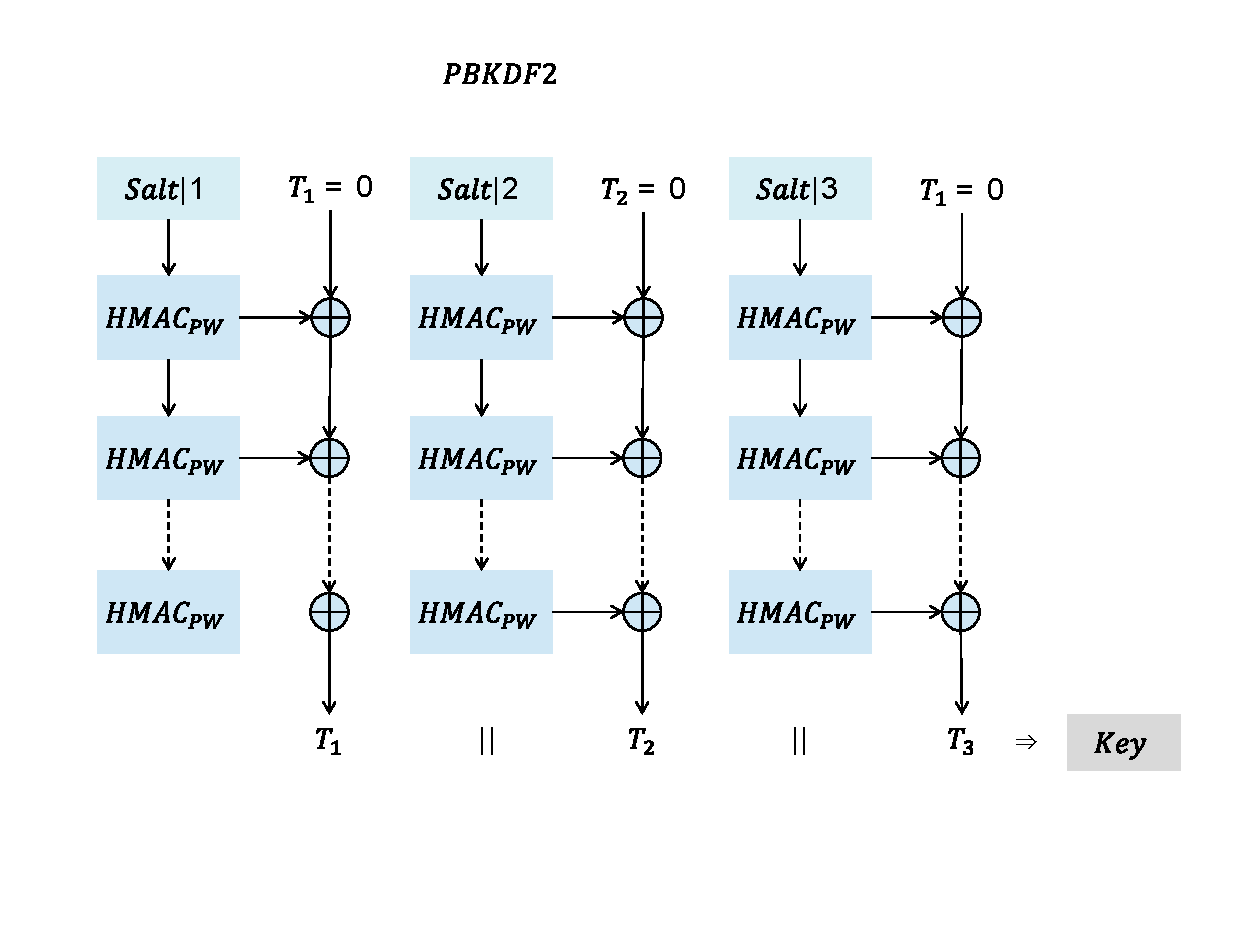
\includegraphics[width=150mm]{./images/PBKDF2}
\caption{The structure of PBKDF2}
\end{figure}

Password Based Key Derivation Function 2 is a KDF, which uses HMAC with SHA1 as a pseudo-random function, which is applied multiple times. It builds the keys from multiple parts depending on the size of the used hash functions output and the desired key size. 
\subsubsection*{Types}
\begin{lstlisting}{}
   package KDF is new Crypto.Symmetric.KDF(return_type        => W_Block512,
                                           security_parameter => Natural,
                                           H                  => Hmac_Package.H);
   type PBKDF2_KDF is new KDF.KDF_Scheme with private;

\end{lstlisting}
PBKDF2 takes salt and password as input, and has the parameters key size and round count. The round count, a natural, is defined by the \texttt{security\_parameter}. The key size is, when using PBKDF2 via the KDF-API, fixed at 512 Bit, but additional functions granting more flexibility are available. \texttt{PBKDF2\_KDF} implements the \texttt{KDF\_Scheme}, containing only the \texttt{security\_parameter}. 

\subsection*{Functions}
\begin{lstlisting}{}
overriding
   procedure Derive(This	: in out PBKDF2_KDF;
                    Salt	: in 	String;
                    Password	: in	String;
                    Key		: out	W_Block512);
   overriding
   procedure Derive(This	: in out PBKDF2_KDF;
                    Salt	: in 	Bytes;
                    Password	: in	Bytes;
                    Key		: out	W_Block512);
   procedure Derive(This	: in out PBKDF2_KDF;
                    Salt	: in 	String;
                    Password	: in	String;
                    Key		: out	Bytes;
                    DK_Len	: in 	Natural);
   procedure Derive(This	: in out PBKDF2_KDF;
                    Salt	: in 	Bytes;
                    Password	: in	Bytes;
                    Key		: out	Bytes;
      		    DK_Len	: in 	Natural);
   overriding
   function Initialize(This	: out PBKDF2_KDF;
                       Parameter: in Natural) return Boolean; 

\end{lstlisting}
\begin{itemize}
	\item The functions \texttt{Derive()} derive a Key from the Input; the first two \texttt{Derive()} are overriding the abstract functions from KDF, the third and fourth are implemented for more flexibility, enabling the user to change the desired derived key length.
	\item The function \texttt{Initialize()} sets the security\_variable, overriding the Initialize function of KDF.
\end{itemize}
The API provides a function for initialization as well as two flavors of key derivation. More Variation may be found in the specific KDFs. 





\section{Sha512crypt}

\begin{figure}[ht!]
\centering
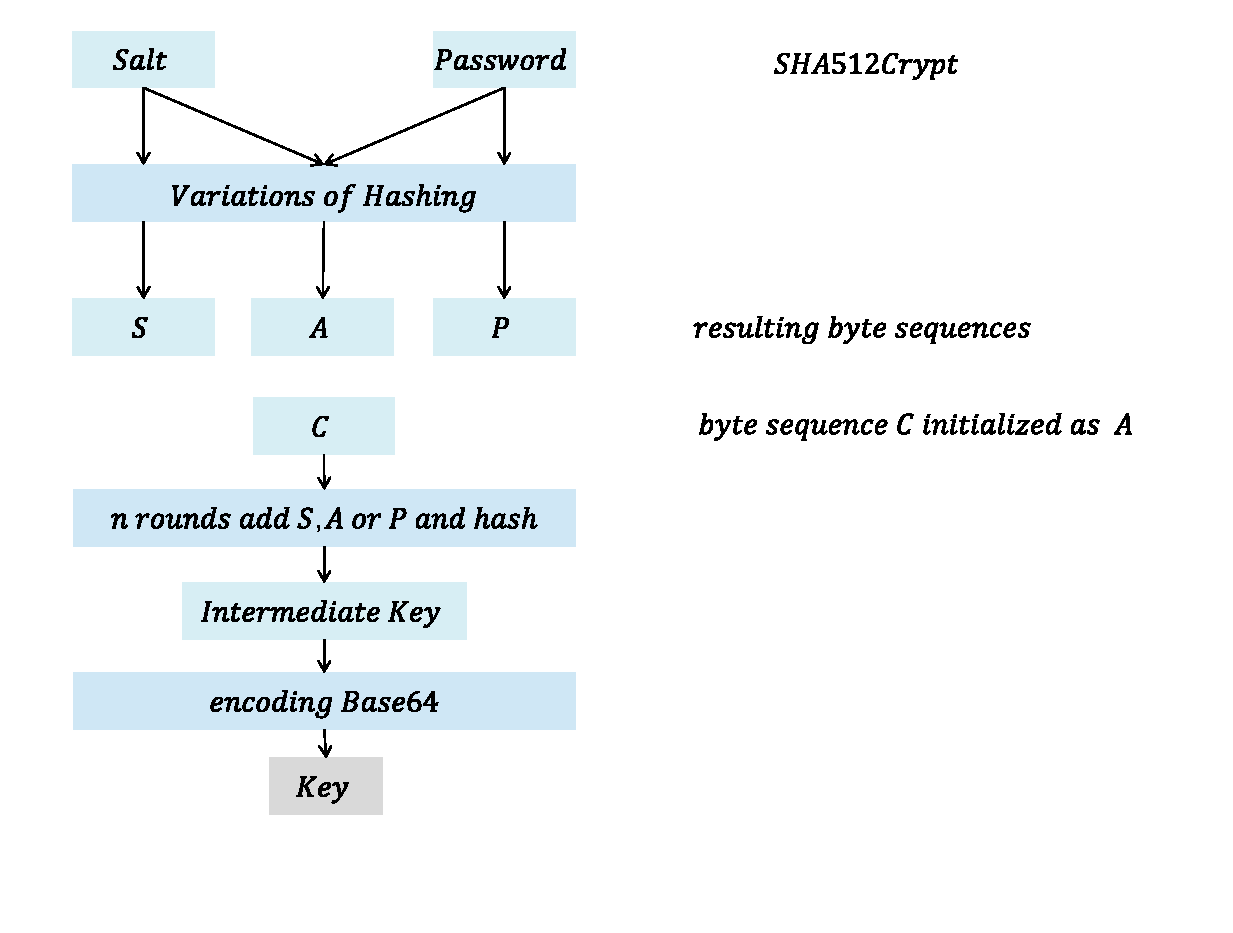
\includegraphics[width=150mm]{./images/SHA512Crypt}
\caption{The structure of SHA512Crypt}
\end{figure}

Sha512Crypt derives a key of a fixed size(86) from a salt and a password string. Those are n, the \texttt{security\_parameter}, rounds long in variations hashed, mixed and concatenated and finally encoded base64.
\subsubsection*{Types}
\begin{lstlisting}{}
   subtype S5C_String is String(1..86) ;

   package KDF is new Crypto.Symmetric.KDF(return_type        => S5C_String,
                                           security_parameter => Natural,
                                           H                  => Crypto.Symmetric.Hashfunction_SHA512);

\end{lstlisting}
Subtype \texttt{S5C\_String} is the fixed-length output string, The round count, a natural, is defined by the \texttt{security\_parameter}. \texttt{SHA512Crypt\_KDF} implements the \texttt{KDF\_Scheme}, containing only the \texttt{security\_parameter}. 

\subsection*{Functions}
\begin{lstlisting}{}
overriding
   procedure Derive(This	: in out SHA512Crypt_KDF;
                    Salt	: in 	String;
                    Password	: in	String;
                    Key		: out	S5C_String);

   overriding
   procedure Derive(This	: in out SHA512Crypt_KDF;
                    Salt	: in 	Bytes;
                    Password	: in	Bytes;
                    Key		: out	S5C_String);

   function Initialize(This	: out SHA512Crypt_KDF;
                       Parameter: in Natural) return Boolean;


\end{lstlisting}
\begin{itemize}
	\item The functions \texttt{Derive()} derive a Key from the Input, overriding the \texttt{KDF} functions.
	\item The function \texttt{Initialize()}, overriding \texttt{Initialize()} from the KDF, sets the \texttt{security\_parameter}.
\end{itemize}


\section{SCrypt}
SCrypt relies on a group of nested functions for deriving a Key from a Salt and a Password Input. It uses the additional parameters Cost Parameter and Parallelization Parameter in the Computation for adjusting the CPU and Memory costs.
\subsubsection*{Types}
\begin{lstlisting}{}
package KDF is new Crypto.Symmetric.KDF(return_type        => W_Block512,
                                           security_parameter => Natural,
                                           H                  => Crypto.Symmetric.Hashfunction_SHA512);

   type Scrypt_KDF is new KDF.KDF_Scheme with private;


\end{lstlisting}

\begin{figure}[ht!]
\centering
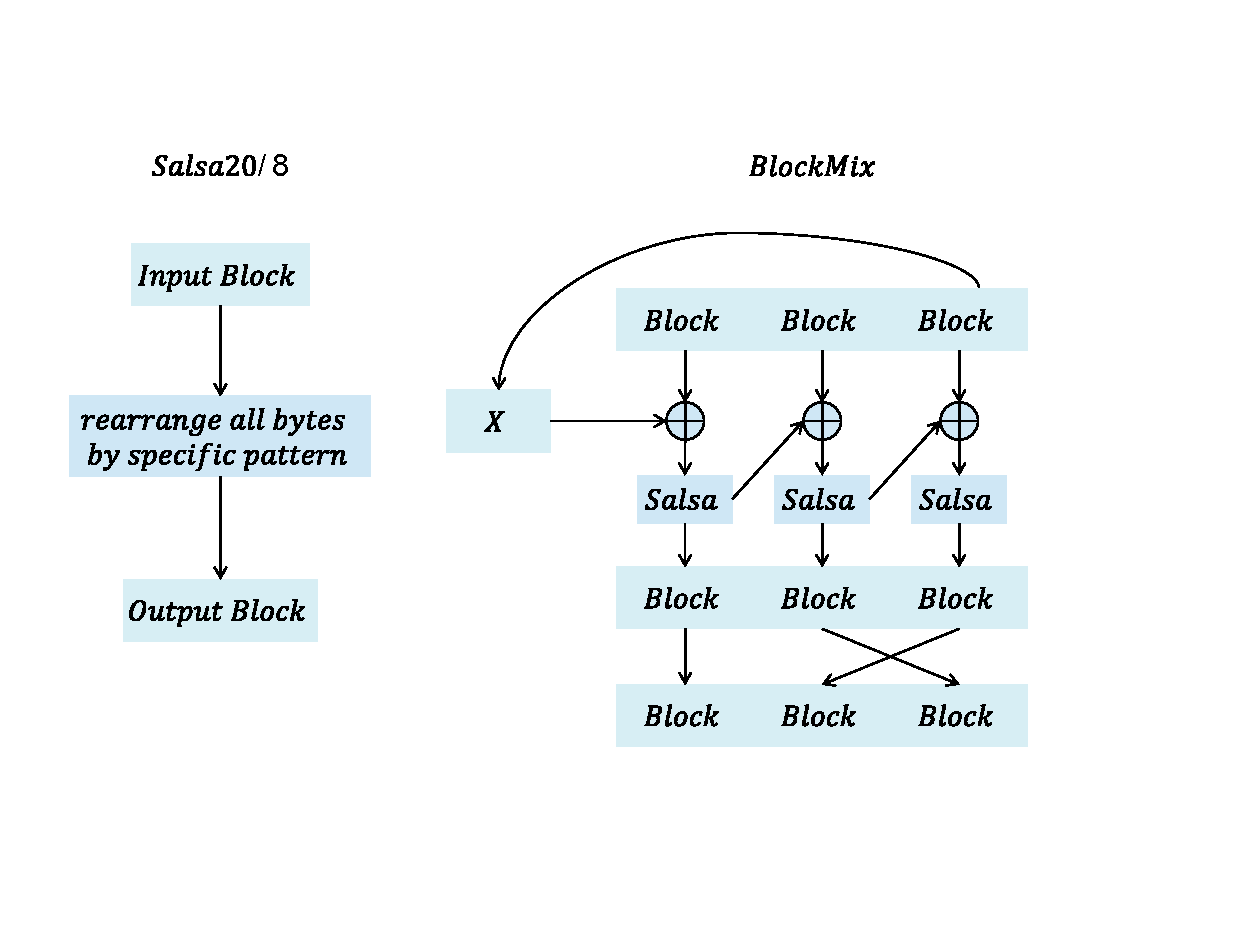
\includegraphics[width=150mm]{./images/Scrypta}
\caption{The structure of SCrypt, part 1}
\end{figure}

\begin{figure}[ht!]
\centering
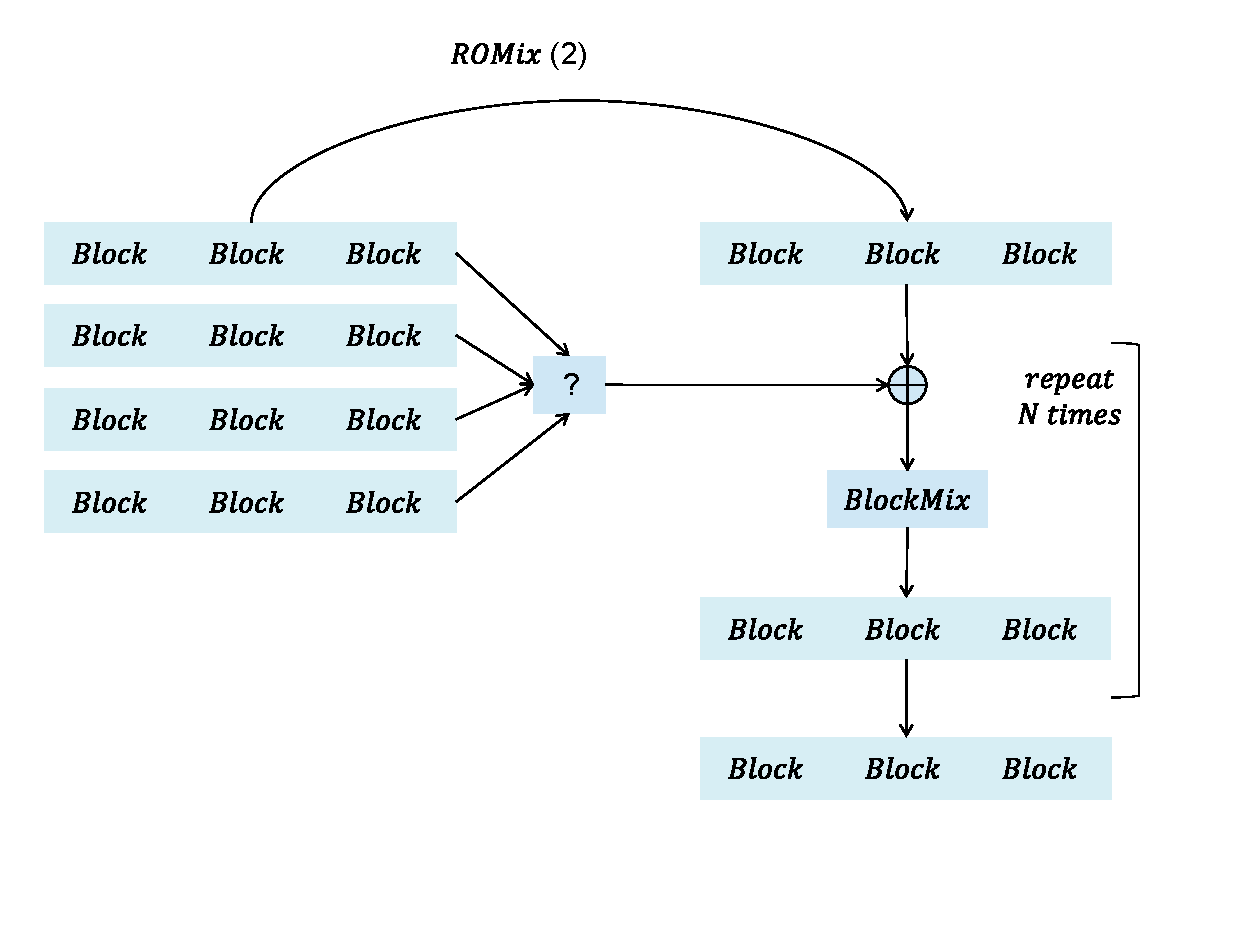
\includegraphics[width=150mm]{./images/Scryptb}
\caption{The structure of SCrypt, part 2}
\end{figure}

\begin{figure}[ht!]
\centering
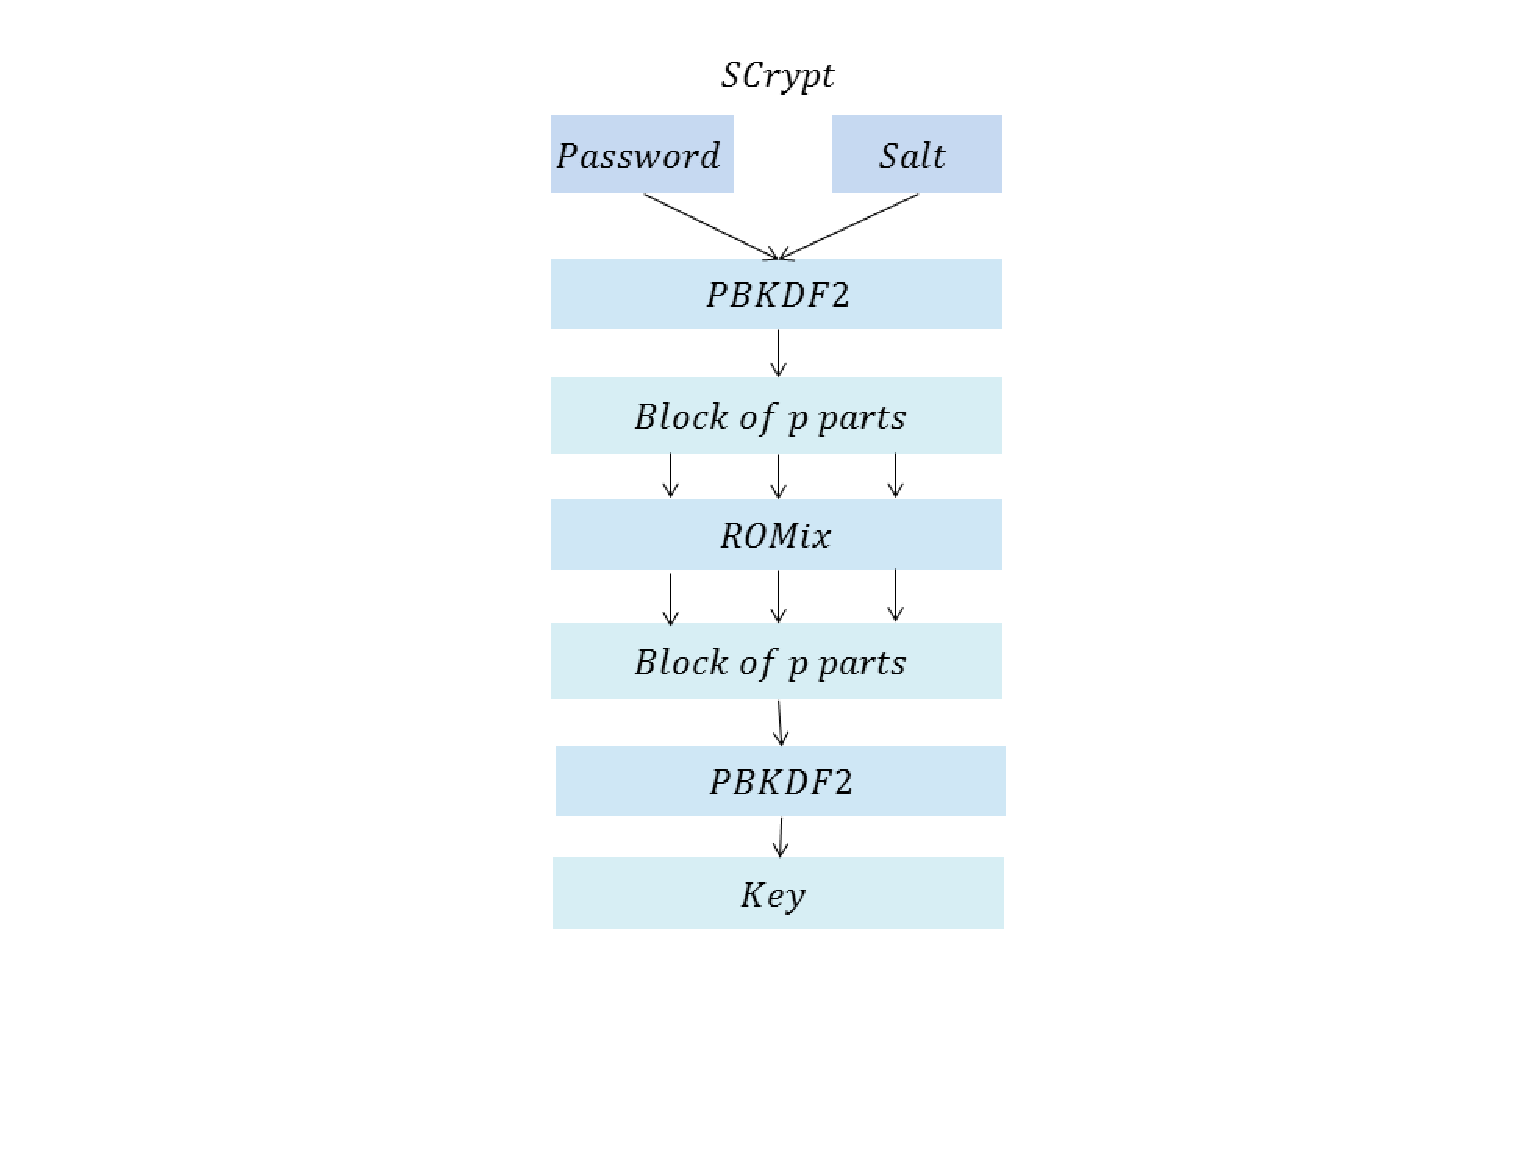
\includegraphics[width=150mm]{./images/Scryptc}
\caption{The structure of SCrypt, part 3}
\end{figure}

Scrypt can return arbitrary key lengthes, but for compatibility with KDF, the \texttt{return\_type} is set to \texttt{W\_Block512}. The \texttt{security\_parameter} relates to the aforementioned Cost Parameter, which must be a power of two – Cost parameter is 2 to the power of \texttt{security\_parameter}.  \texttt{Scrypt\_KDF} implements the \texttt{KDF\_Scheme}, containing only the \texttt{security\_parameter}.

\subsection*{Functions}
\begin{lstlisting}{}
overriding
   procedure Derive(This	: in out Scrypt_KDF;
                    Salt	: in 	String;
                    Password	: in	String;
                    Key		: out	W_Block512);

   overriding
   procedure Derive(This	: in out Scrypt_KDF;
                    Salt	: in 	Bytes;
                    Password	: in	Bytes;
                    Key		: out	W_Block512);

   overriding
   function Initialize(This	: out Scrypt_KDF;
                       Parameter: in Natural) return Boolean;


   procedure scrypt (Password 	: in 	String;
                     Salt 	: in 	String;
                     r		: in 	Natural;
                     N		: in 	Natural;
                     p		: in	Natural;
                     dkLen	: in	Natural;
                     Key	: out 	Bytes);

\end{lstlisting}
\begin{itemize}
	\item The functions \texttt{Derive()} derive a Key from the Input, overriding the KDF functions.
	\item The function \texttt{Initialize()}, overriding \texttt{Initialize()} from \texttt{KDF}, sets the \texttt{security\_parameter}.
	\item The procedure \texttt{scrypt()} offers the complete scrypt implementation, enabling the user to set all parameters provided by the algorithm.
\end{itemize}

